\chapter{Results and Discussion}

\section{Introduction}

Chapter 4 described the implementation methodology used to prepare datasets, train YOLO segmentation models, evaluate checkpoints, and collect experiment outputs. This chapter presents the experimental results and discusses the main findings. The analysis focuses on how segmentation performance changes when the training strategy moves from EO-only learning to supervised IR and mixed EO+IR learning, and then to larger models, higher input resolution, and ensembling.

The primary evaluation setting is IR-only validation because the central problem is improving segmentation quality in the IR domain. The combined EO+IR validation setting is used as a secondary measure of cross-modality robustness. The main metric is mask mAP50-95 because it is stricter than mask mAP50 and better reflects segmentation quality across different overlap thresholds.

\section{Result Organization}

The results are reported using the unified experiment notation introduced in Chapter 3. The experiments are grouped as follows:

\begin{itemize}
    \item E01-E04: EO-only and grayscale-domain baselines.
    \item E05-E07: supervised YOLO11s experiments using EO+IR, IR-only, and balanced EO+IR training.
    \item E08-E09: YOLO11l model scaling experiments.
    \item E10: mask-aware ensemble evaluation.
    \item E11-E12: high-resolution YOLO11l and YOLO11x experiments.
\end{itemize}

Figures in this chapter are designed to summarize the same results from different viewpoints. If the generated figure files are not yet available, the document shows a placeholder box with the intended filename.

\begin{figure}[htbp]
\centering
\IfFileExists{Figures/Chapter5/performance_progression_story.png}{%
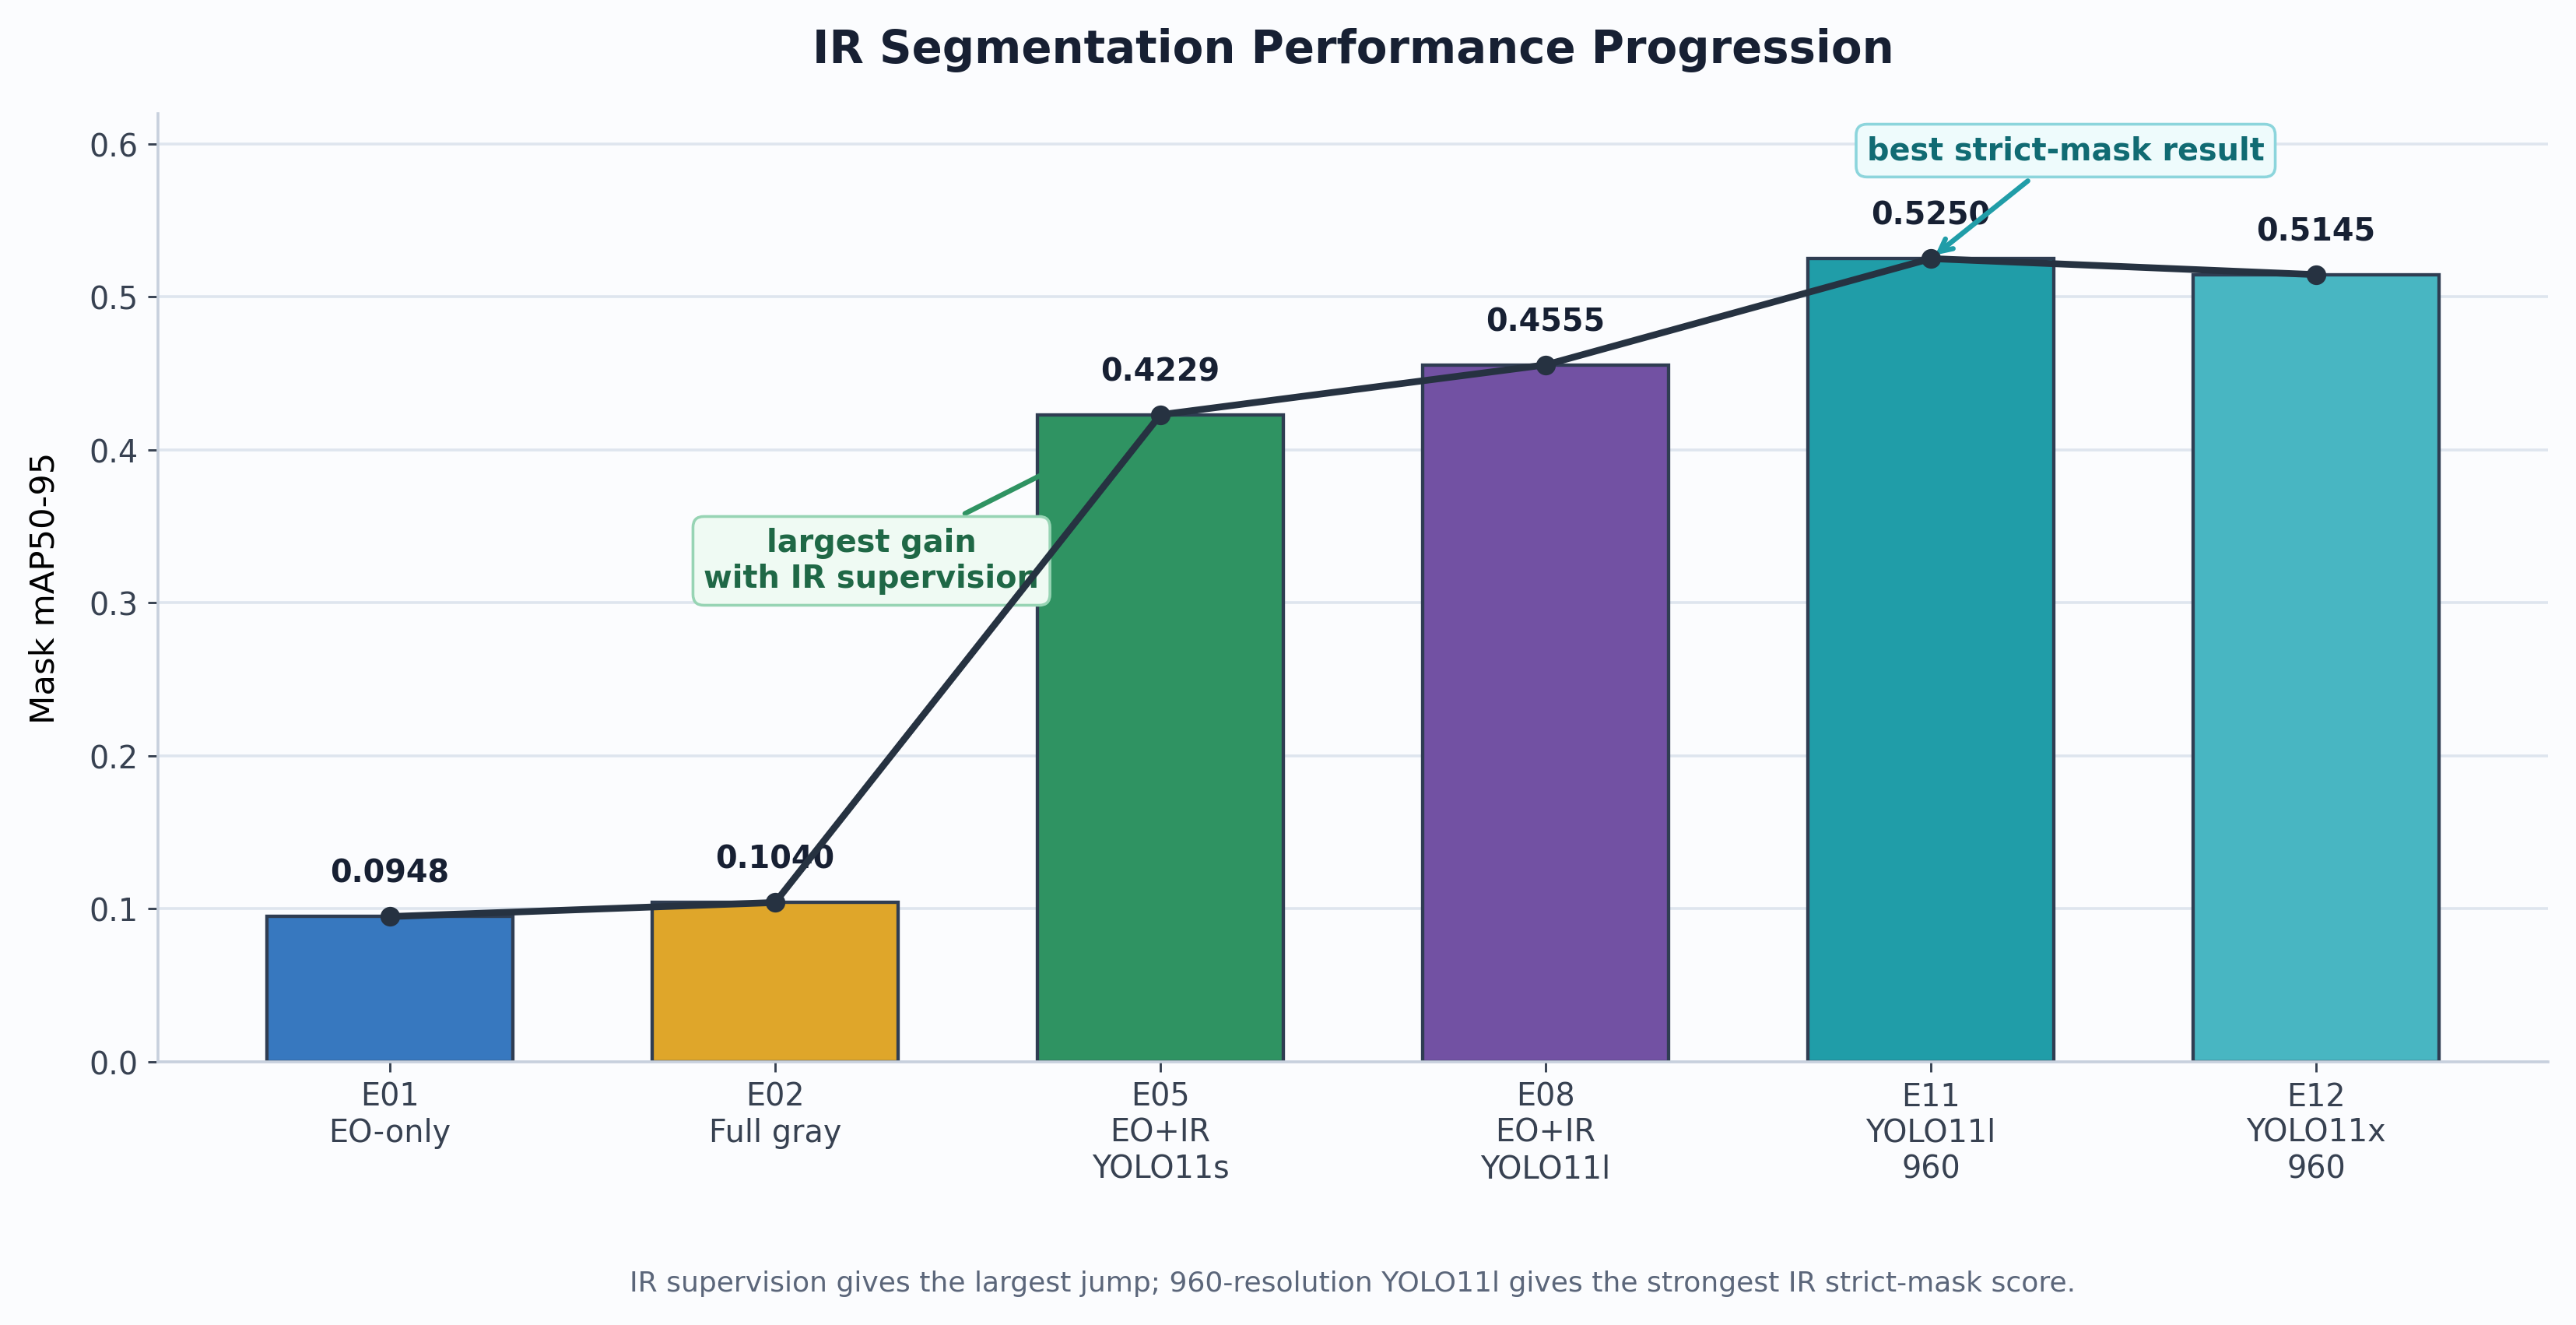
\includegraphics[width=\textwidth]{Figures/Chapter5/performance_progression_story.png}%
}{%
\fbox{\parbox{0.92\textwidth}{\centering Placeholder for \texttt{performance\_progression\_story.png}}}%
}
\caption{Performance progression on IR-only validation using strict mask mAP50-95.}
\label{fig:performance_progression_story}
\end{figure}

\section{EO-only and Grayscale-domain Baselines}

The first experiment group evaluates whether EO-only training can transfer directly to IR segmentation. E01 is the direct EO-only baseline. E02, E03, and E04 apply grayscale-domain transformations to EO training images before evaluating on IR validation.

Table \ref{tab:eo_only_ir_results} shows that the EO-only and grayscale-domain baselines remain weak on IR segmentation. E01 obtains a mask mAP50-95 of 0.0948 on IR validation. Full grayscale conversion in E02 improves this slightly to 0.1040, but the improvement is small. Box-guided grayscale and mask-guided grayscale do not improve strict IR mask quality over the EO-only baseline.

\begin{table}[h]
\centering
\caption{EO-only and grayscale-domain baseline results on IR validation.}
\label{tab:eo_only_ir_results}
\begin{tabular}{llllr}
\hline
\textbf{ID} & \textbf{Training Strategy} & \textbf{Model} & \textbf{Training Data} & \textbf{Mask mAP50-95} \\
\hline
E01 & EO-only baseline & YOLO11s-seg & EO & 0.0948 \\
E02 & Full grayscale EO & YOLO11s-seg & EO gray & 0.1040 \\
E03 & Box-guided grayscale EO & YOLO11s-seg & EO box-gray & 0.0811 \\
E04 & Mask-guided grayscale EO & YOLO11s-seg & EO mask-gray & 0.0812 \\
\hline
\end{tabular}
\end{table}

\begin{figure}[htbp]
\centering
\IfFileExists{Figures/Chapter5/eo_only_augmentation_comparison.png}{%
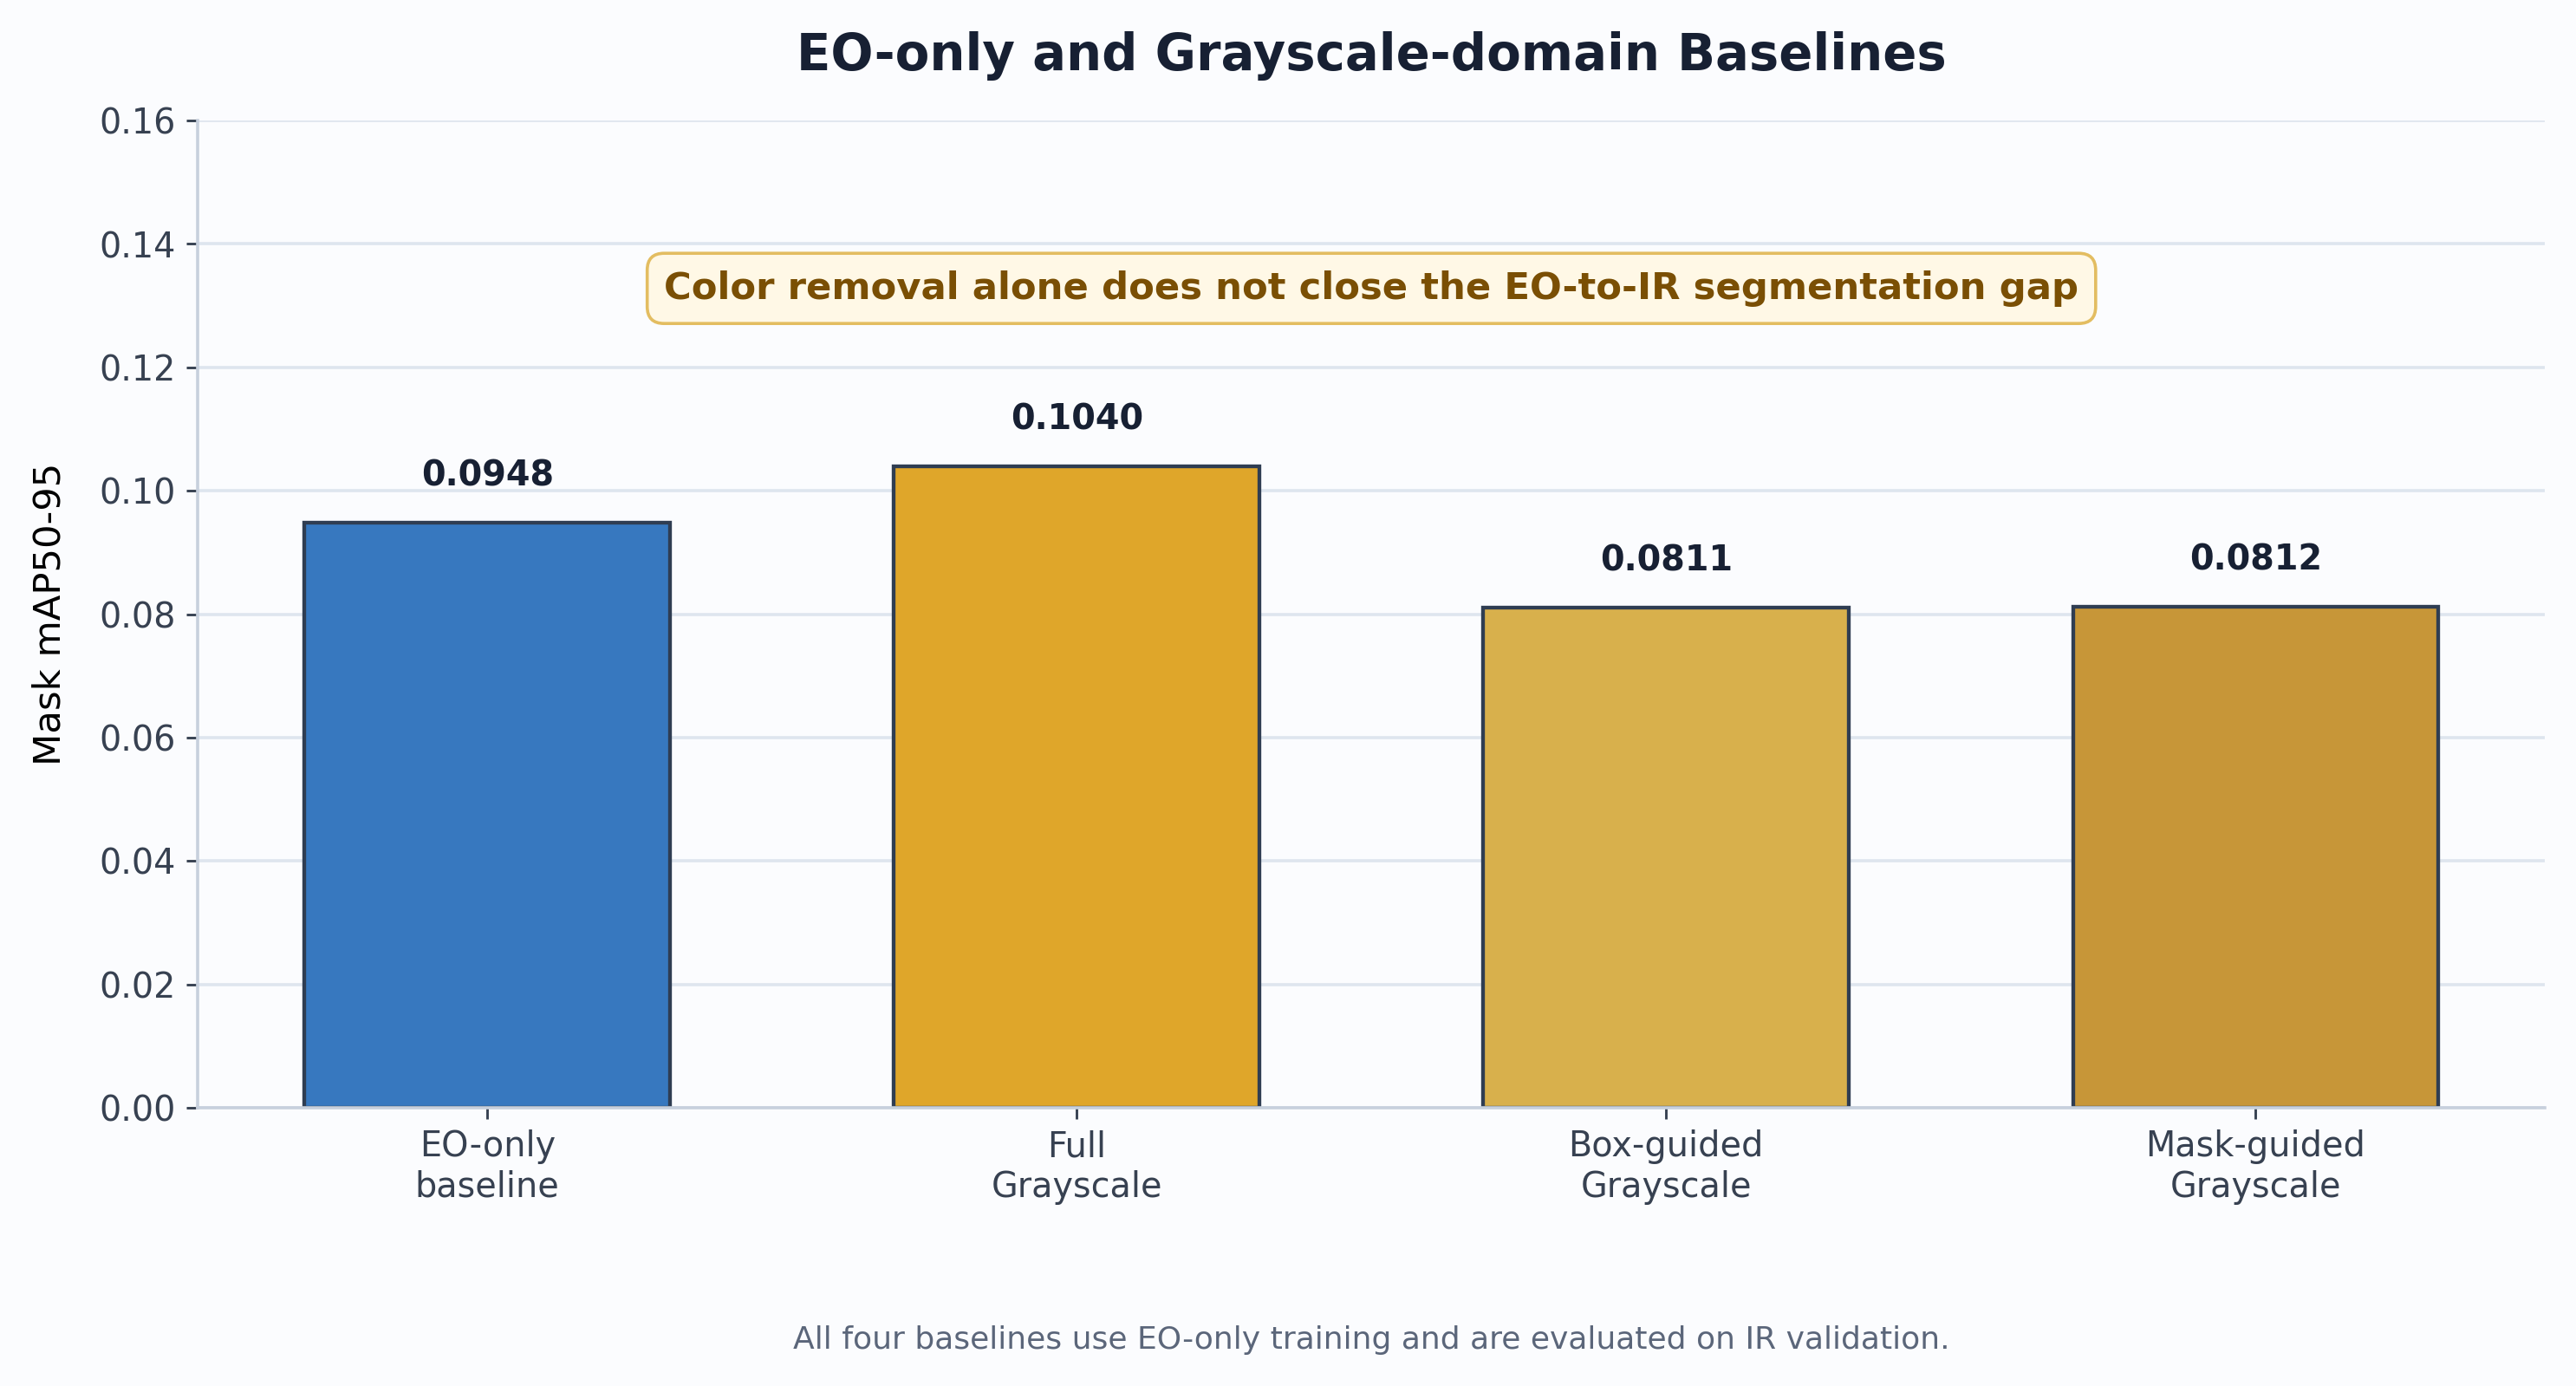
\includegraphics[width=\textwidth]{Figures/Chapter5/eo_only_augmentation_comparison.png}%
}{%
\fbox{\parbox{0.92\textwidth}{\centering Placeholder for \texttt{eo\_only\_augmentation\_comparison.png}}}%
}
\caption{Comparison of EO-only and grayscale-domain baselines on IR validation.}
\label{fig:eo_only_augmentation_comparison}
\end{figure}

These results indicate that removing visible color cues from EO imagery is not sufficient to close the EO-to-IR segmentation gap. The model still lacks real IR appearance information, especially thermal contrast, IR boundary behavior, and IR-specific object texture.

\section{Effect of IR Supervision}

The next experiment group introduces real IR supervision. E05 uses joint EO+IR training, E06 uses IR-only training, and E07 uses balanced EO+IR training. These experiments are compared with E01 to measure the effect of adding IR labels.

The improvement is substantial. On IR validation, E01 obtains a mask mAP50-95 of 0.0948, while E05 improves to 0.4229. E06 reaches 0.4342, showing that target-domain IR supervision is highly effective. E07 obtains 0.4031, which is lower than E05 and E06 on IR-only validation, but remains much stronger than EO-only training.

\begin{table}[h]
\centering
\caption{Effect of supervised IR information on mask mAP50-95.}
\label{tab:supervision_results}
\begin{tabular}{llllrr}
\hline
\textbf{ID} & \textbf{Training Strategy} & \textbf{Model} & \textbf{Training Data} & \textbf{IR} & \textbf{EO+IR} \\
\hline
E01 & EO-only baseline & YOLO11s-seg & EO & 0.0948 & 0.1669 \\
E05 & Joint EO+IR & YOLO11s-seg & EO+IR & 0.4229 & 0.3069 \\
E06 & IR-only supervised & YOLO11s-seg & IR & 0.4342 & 0.1902 \\
E07 & Balanced EO+IR & YOLO11s-seg & EO+IR balanced & 0.4031 & 0.2969 \\
\hline
\end{tabular}
\end{table}

\begin{figure}[htbp]
\centering
\IfFileExists{Figures/Chapter5/supervision_strategy_comparison.png}{%
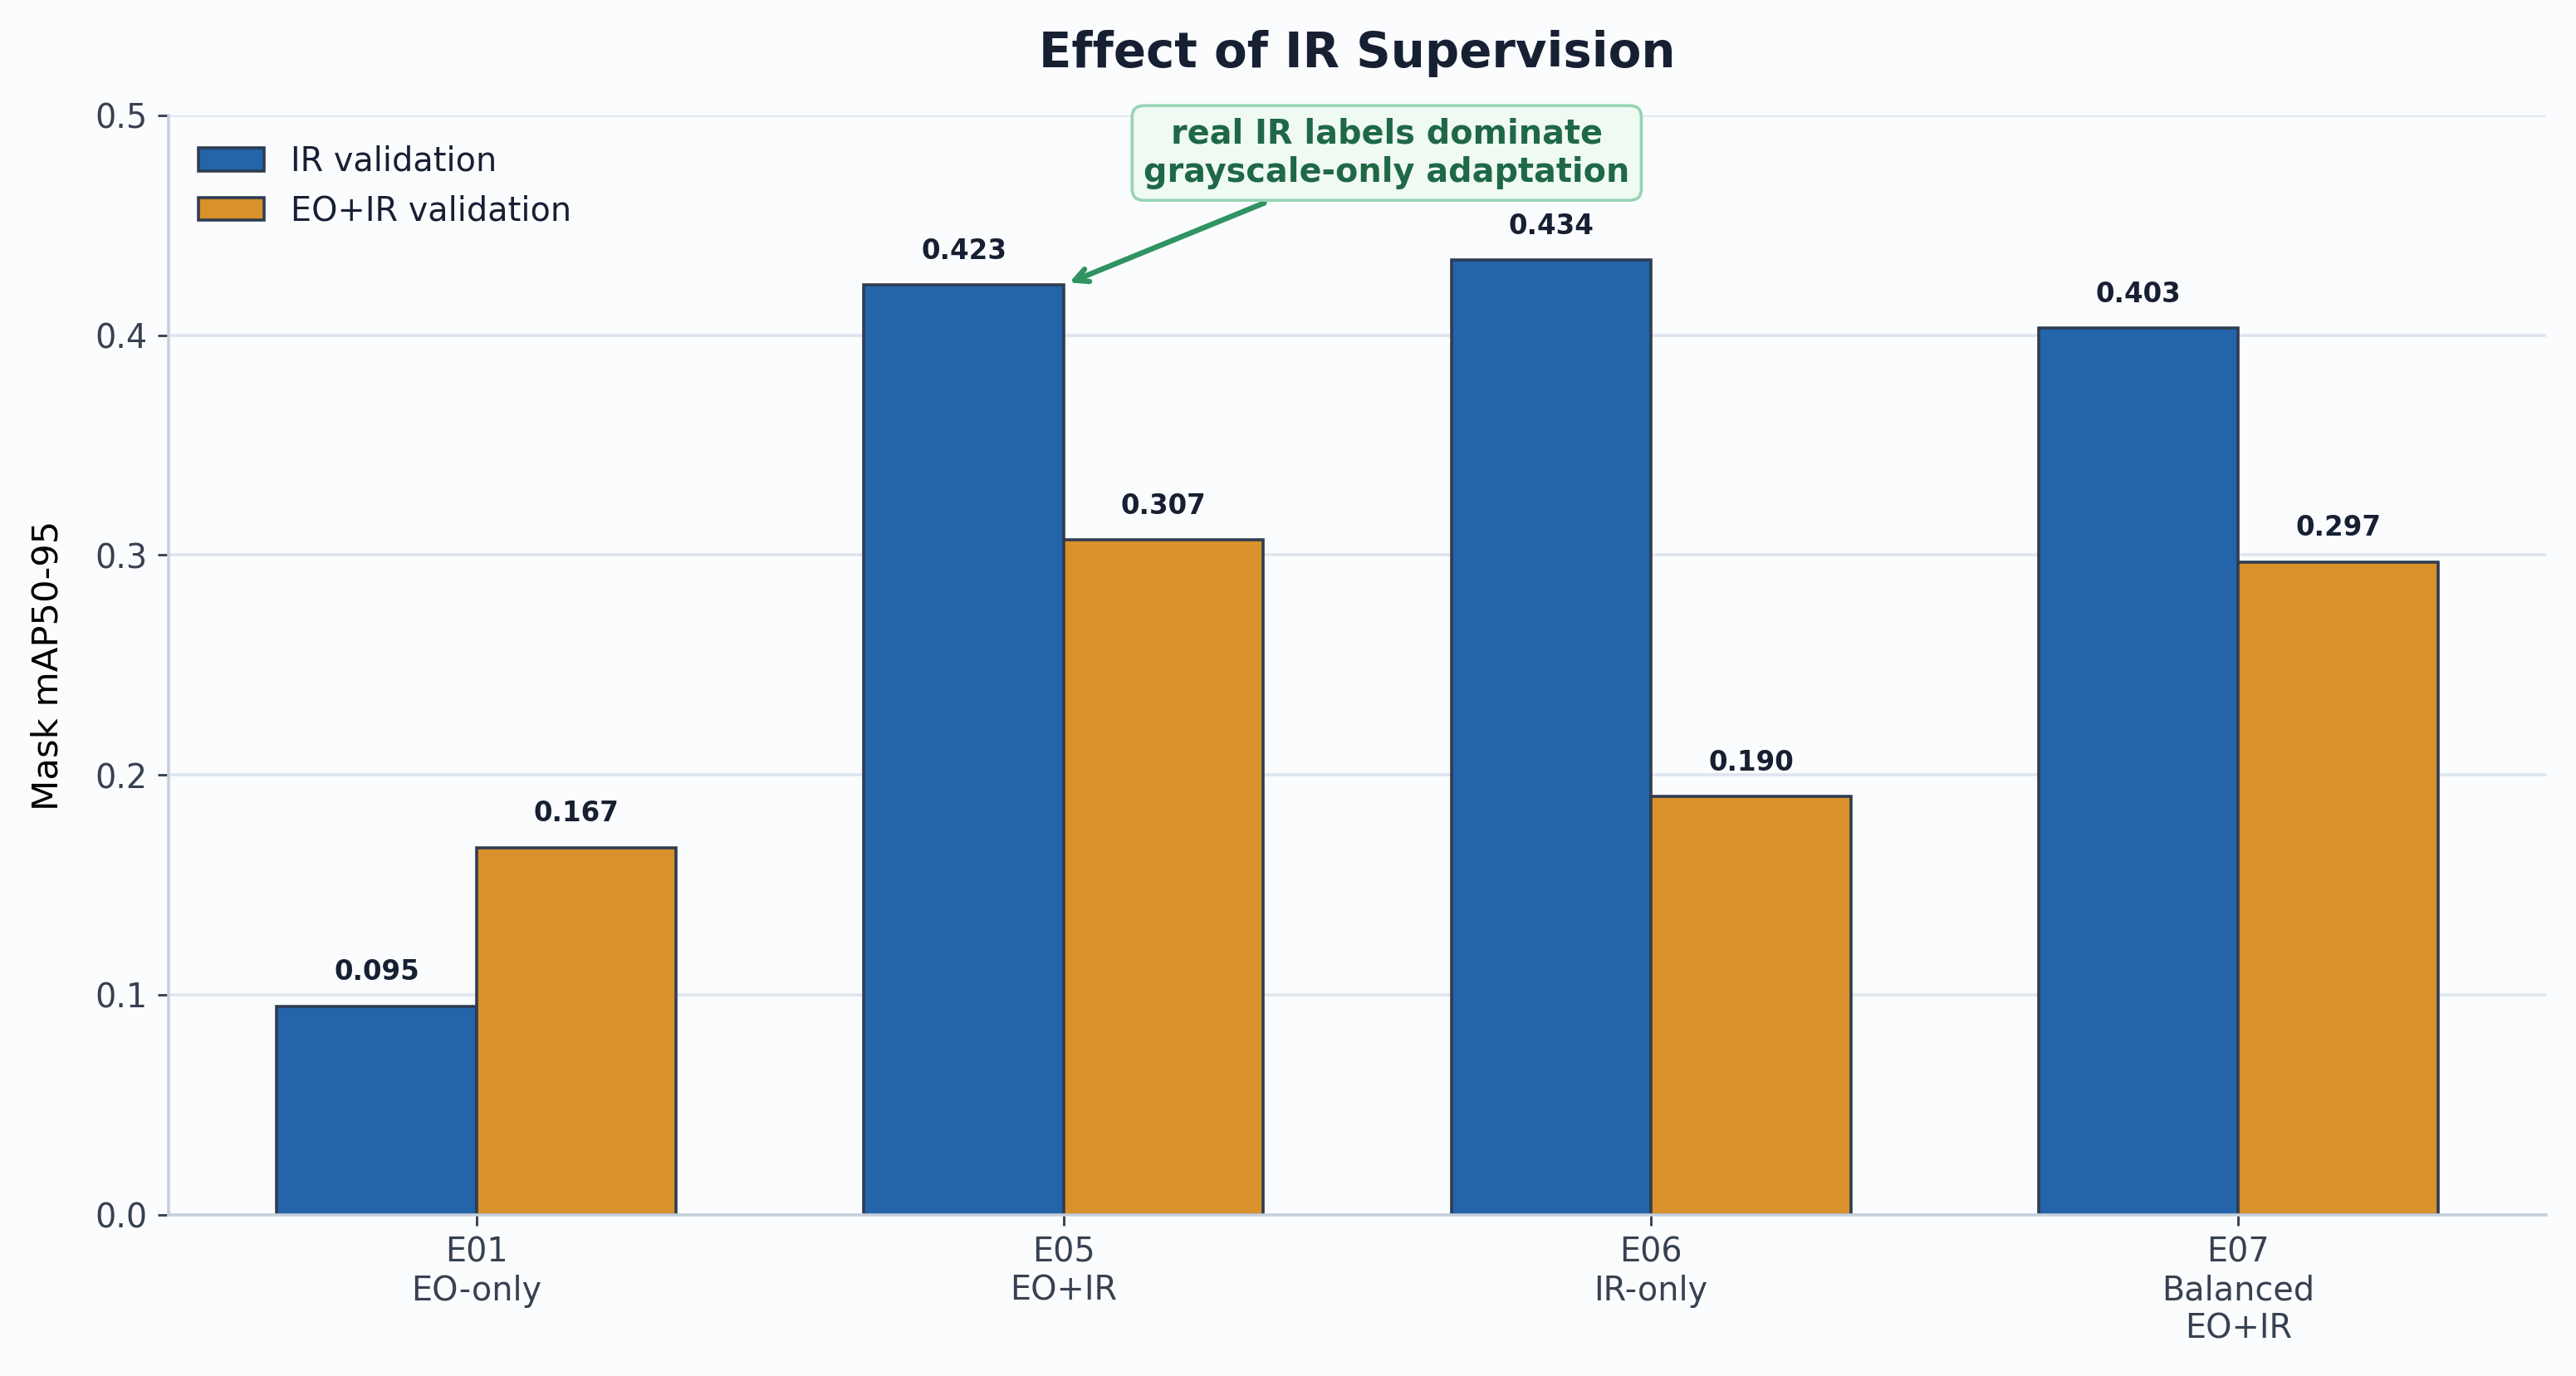
\includegraphics[width=\textwidth]{Figures/Chapter5/supervision_strategy_comparison.png}%
}{%
\fbox{\parbox{0.92\textwidth}{\centering Placeholder for \texttt{supervision\_strategy\_comparison.png}}}%
}
\caption{Effect of adding real IR supervision compared with EO-only training.}
\label{fig:supervision_strategy_comparison}
\end{figure}

The comparison shows that IR supervision is the dominant factor in improving IR segmentation. EO-only transformations provide only limited gains, while real IR labels allow the model to learn modality-specific visual patterns.

\section{Model Scaling Results}

After establishing the importance of IR supervision, the next comparison studies model capacity. E05 and E08 use joint EO+IR training at 640 resolution, but E05 uses YOLO11s-seg and E08 uses YOLO11l-seg. Similarly, E06 and E09 compare IR-only training with YOLO11s-seg and YOLO11l-seg.

On IR validation, E05 achieves 0.4229 mask mAP50-95, while E08 improves to 0.4555. This indicates that increasing model capacity improves mixed-domain segmentation. For IR-only training, E06 achieves 0.4342 and E09 reaches 0.4438. The gain is smaller than in the mixed-domain case, but it still shows that the larger model has useful representational capacity.

\begin{table}[h]
\centering
\caption{Model scaling comparison at 640 resolution.}
\label{tab:model_scaling_results}
\begin{tabular}{llllr}
\hline
\textbf{ID} & \textbf{Training Strategy} & \textbf{Model} & \textbf{Training Data} & \textbf{IR Mask mAP50-95} \\
\hline
E05 & Joint EO+IR & YOLO11s-seg & EO+IR & 0.4229 \\
E08 & Joint EO+IR large & YOLO11l-seg & EO+IR & 0.4555 \\
E06 & IR-only supervised & YOLO11s-seg & IR & 0.4342 \\
E09 & IR-only large & YOLO11l-seg & IR & 0.4438 \\
\hline
\end{tabular}
\end{table}

The scaling results support the use of larger YOLO segmentation models for EO/IR aerial imagery. However, model scaling alone does not provide the strongest improvement. The later high-resolution experiments show a larger gain in strict mask quality.

\section{High-resolution Training Results}

High-resolution training is evaluated using E11 and E12. E11 uses YOLO11l-seg with 960 image size, while E12 uses YOLO11x-seg with 960 image size. These experiments are compared with E08, which uses YOLO11l-seg at 640 resolution.

E08 obtains 0.4555 mask mAP50-95 on IR validation. Increasing the input size to 960 in E11 improves this to 0.5250. This is the strongest primary IR result in the experiment set. E12 obtains 0.5145 on IR validation, which is slightly below E11, but it reaches the best combined EO+IR score of 0.4422.

\begin{figure}[htbp]
\centering
\IfFileExists{Figures/Chapter5/scale_resolution_ablation.png}{%
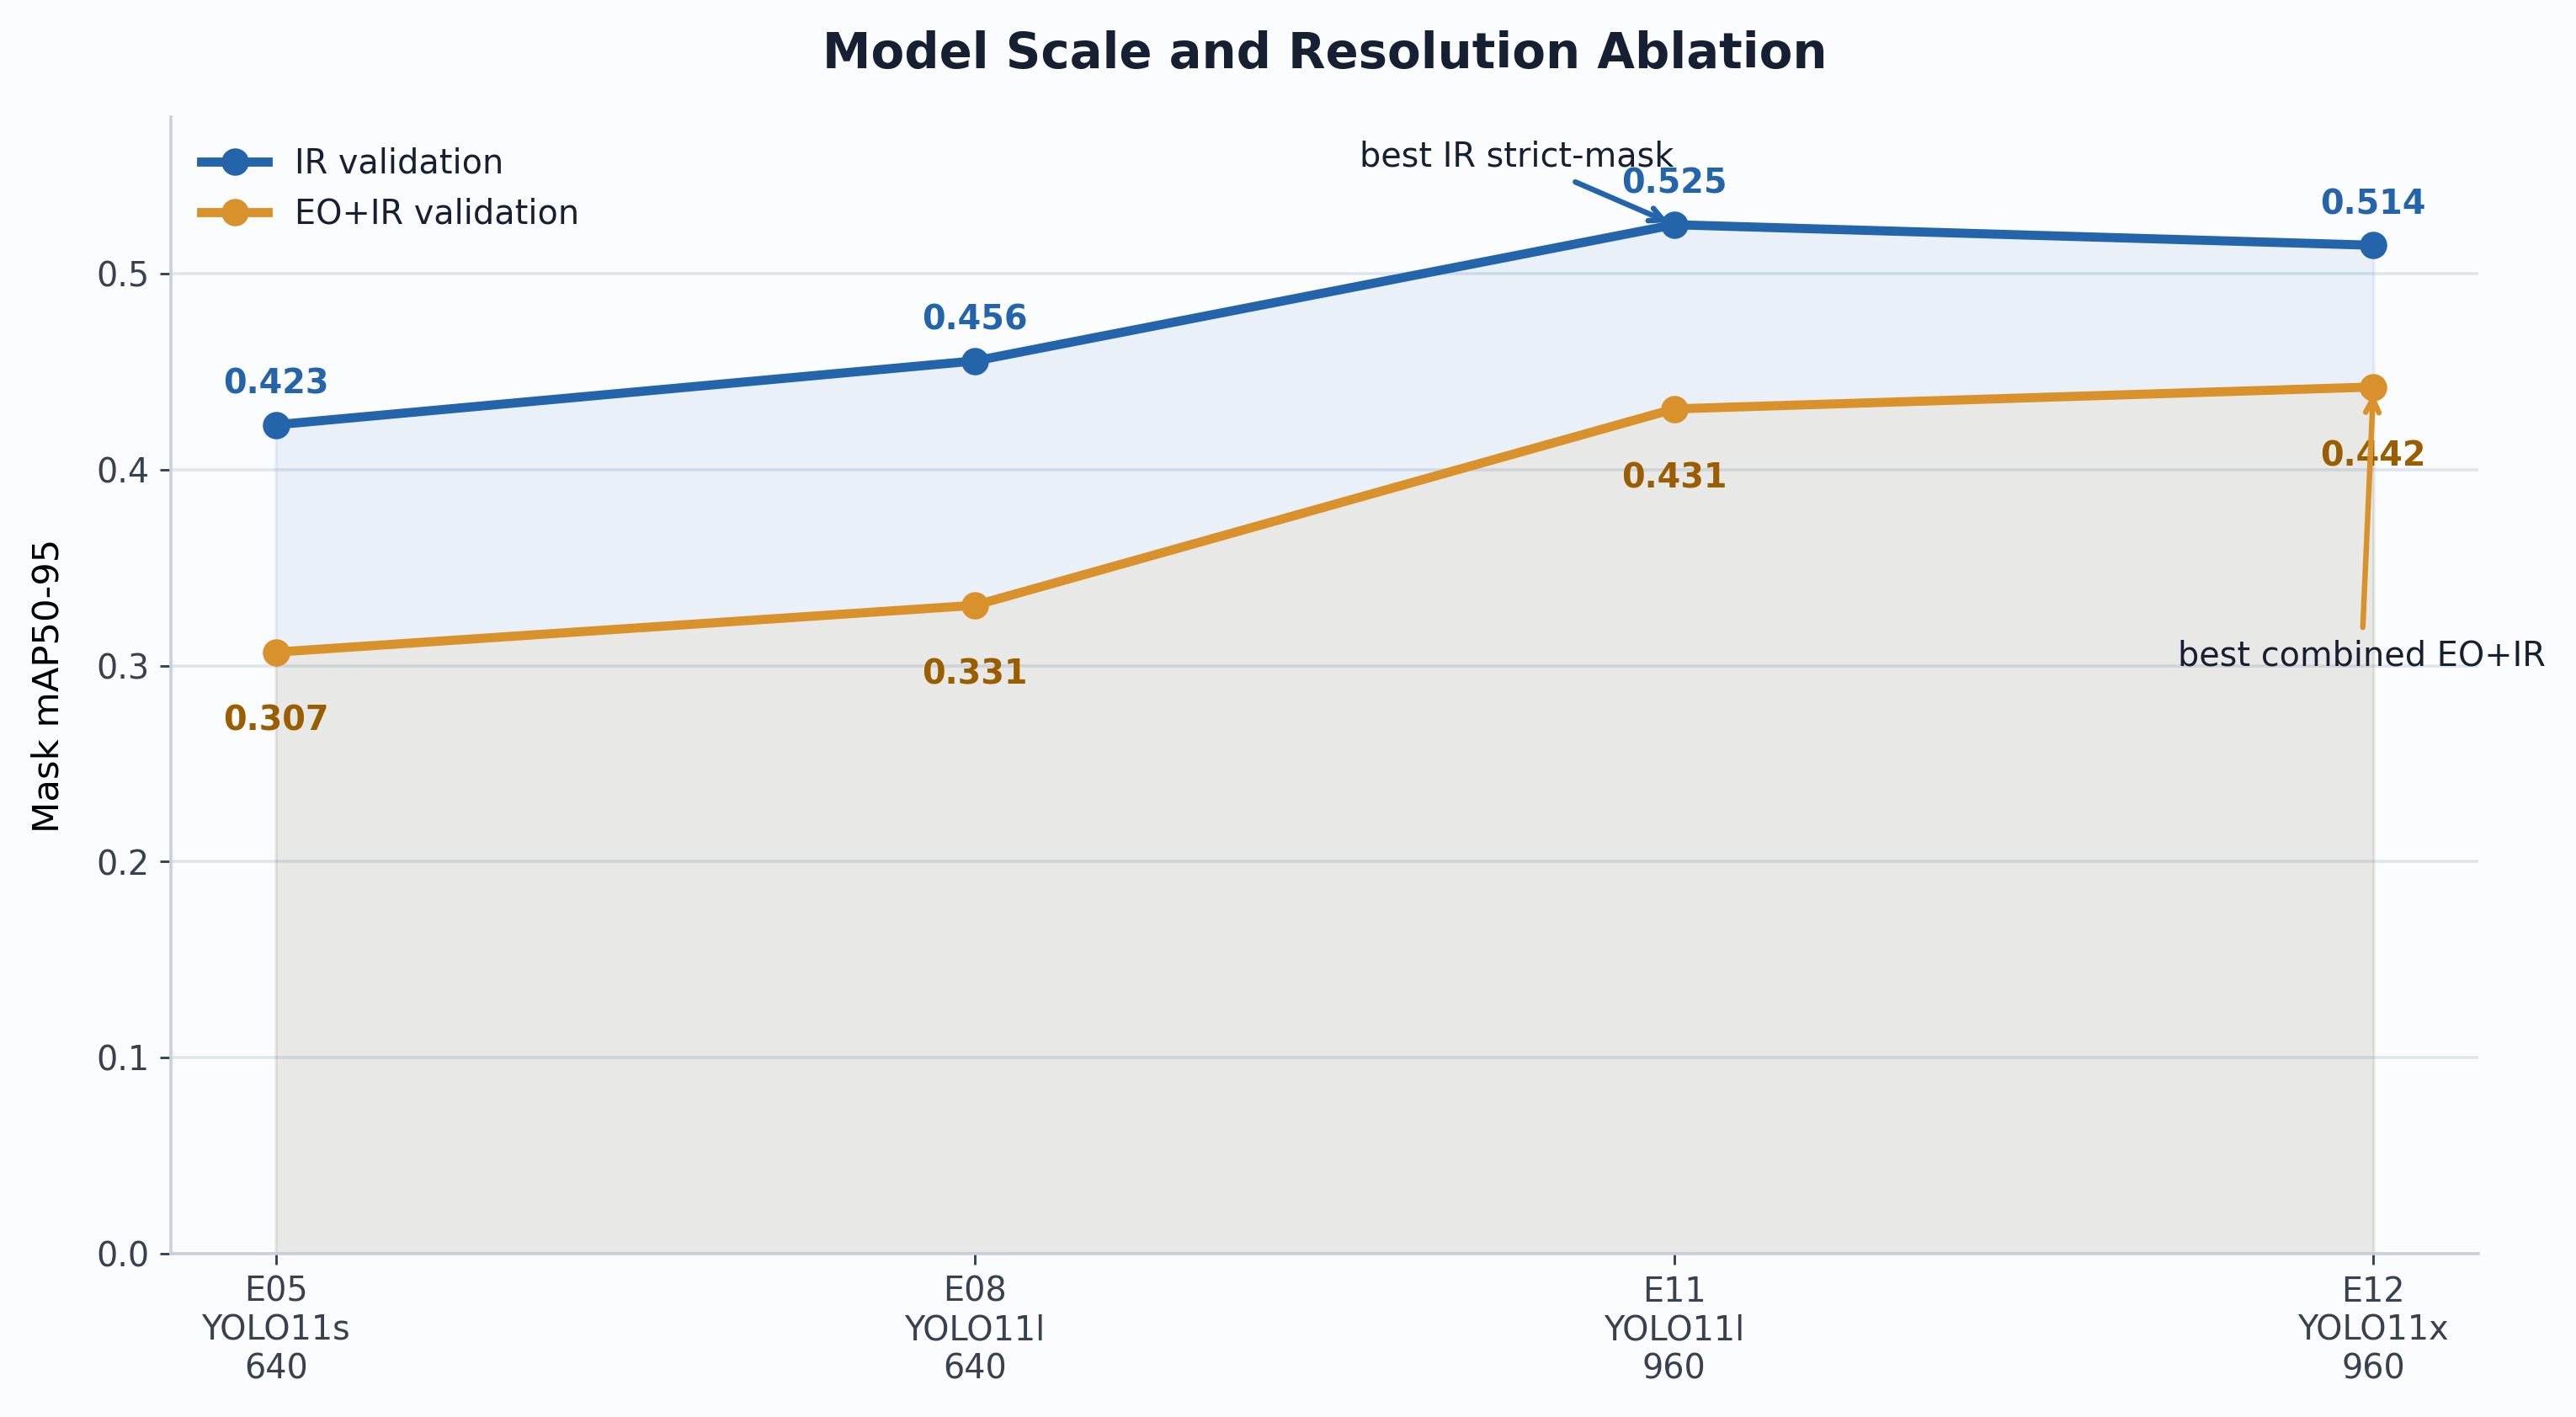
\includegraphics[width=\textwidth]{Figures/Chapter5/scale_resolution_ablation.png}%
}{%
\fbox{\parbox{0.92\textwidth}{\centering Placeholder for \texttt{scale\_resolution\_ablation.png}}}%
}
\caption{Effect of model scale and input resolution on strict mask performance.}
\label{fig:scale_resolution_ablation}
\end{figure}

The high-resolution results indicate that preserving spatial detail is important for aerial segmentation. Many traffic objects are small, and higher image resolution helps the model retain object boundary and shape information. E11 is therefore the preferred model when the primary target is IR-only strict mask quality, while E12 is preferred when combined EO+IR robustness is the main objective.

\section{Ensemble Ablation}

E10 evaluates a mask-aware ensemble using the large mixed-domain model and the large IR-specialist model. The purpose is to test whether late-stage prediction fusion improves beyond strong individual models.

The ensemble obtains 0.4553 mask mAP50-95 on IR validation, which is almost identical to E08 at 0.4555. However, it does not improve over E11 at 0.5250. On combined EO+IR validation, E10 obtains 0.3139, which is below E08 at 0.3308 and below the high-resolution models.

\begin{figure}[htbp]
\centering
\IfFileExists{Figures/Chapter5/ensemble_ablation.png}{%
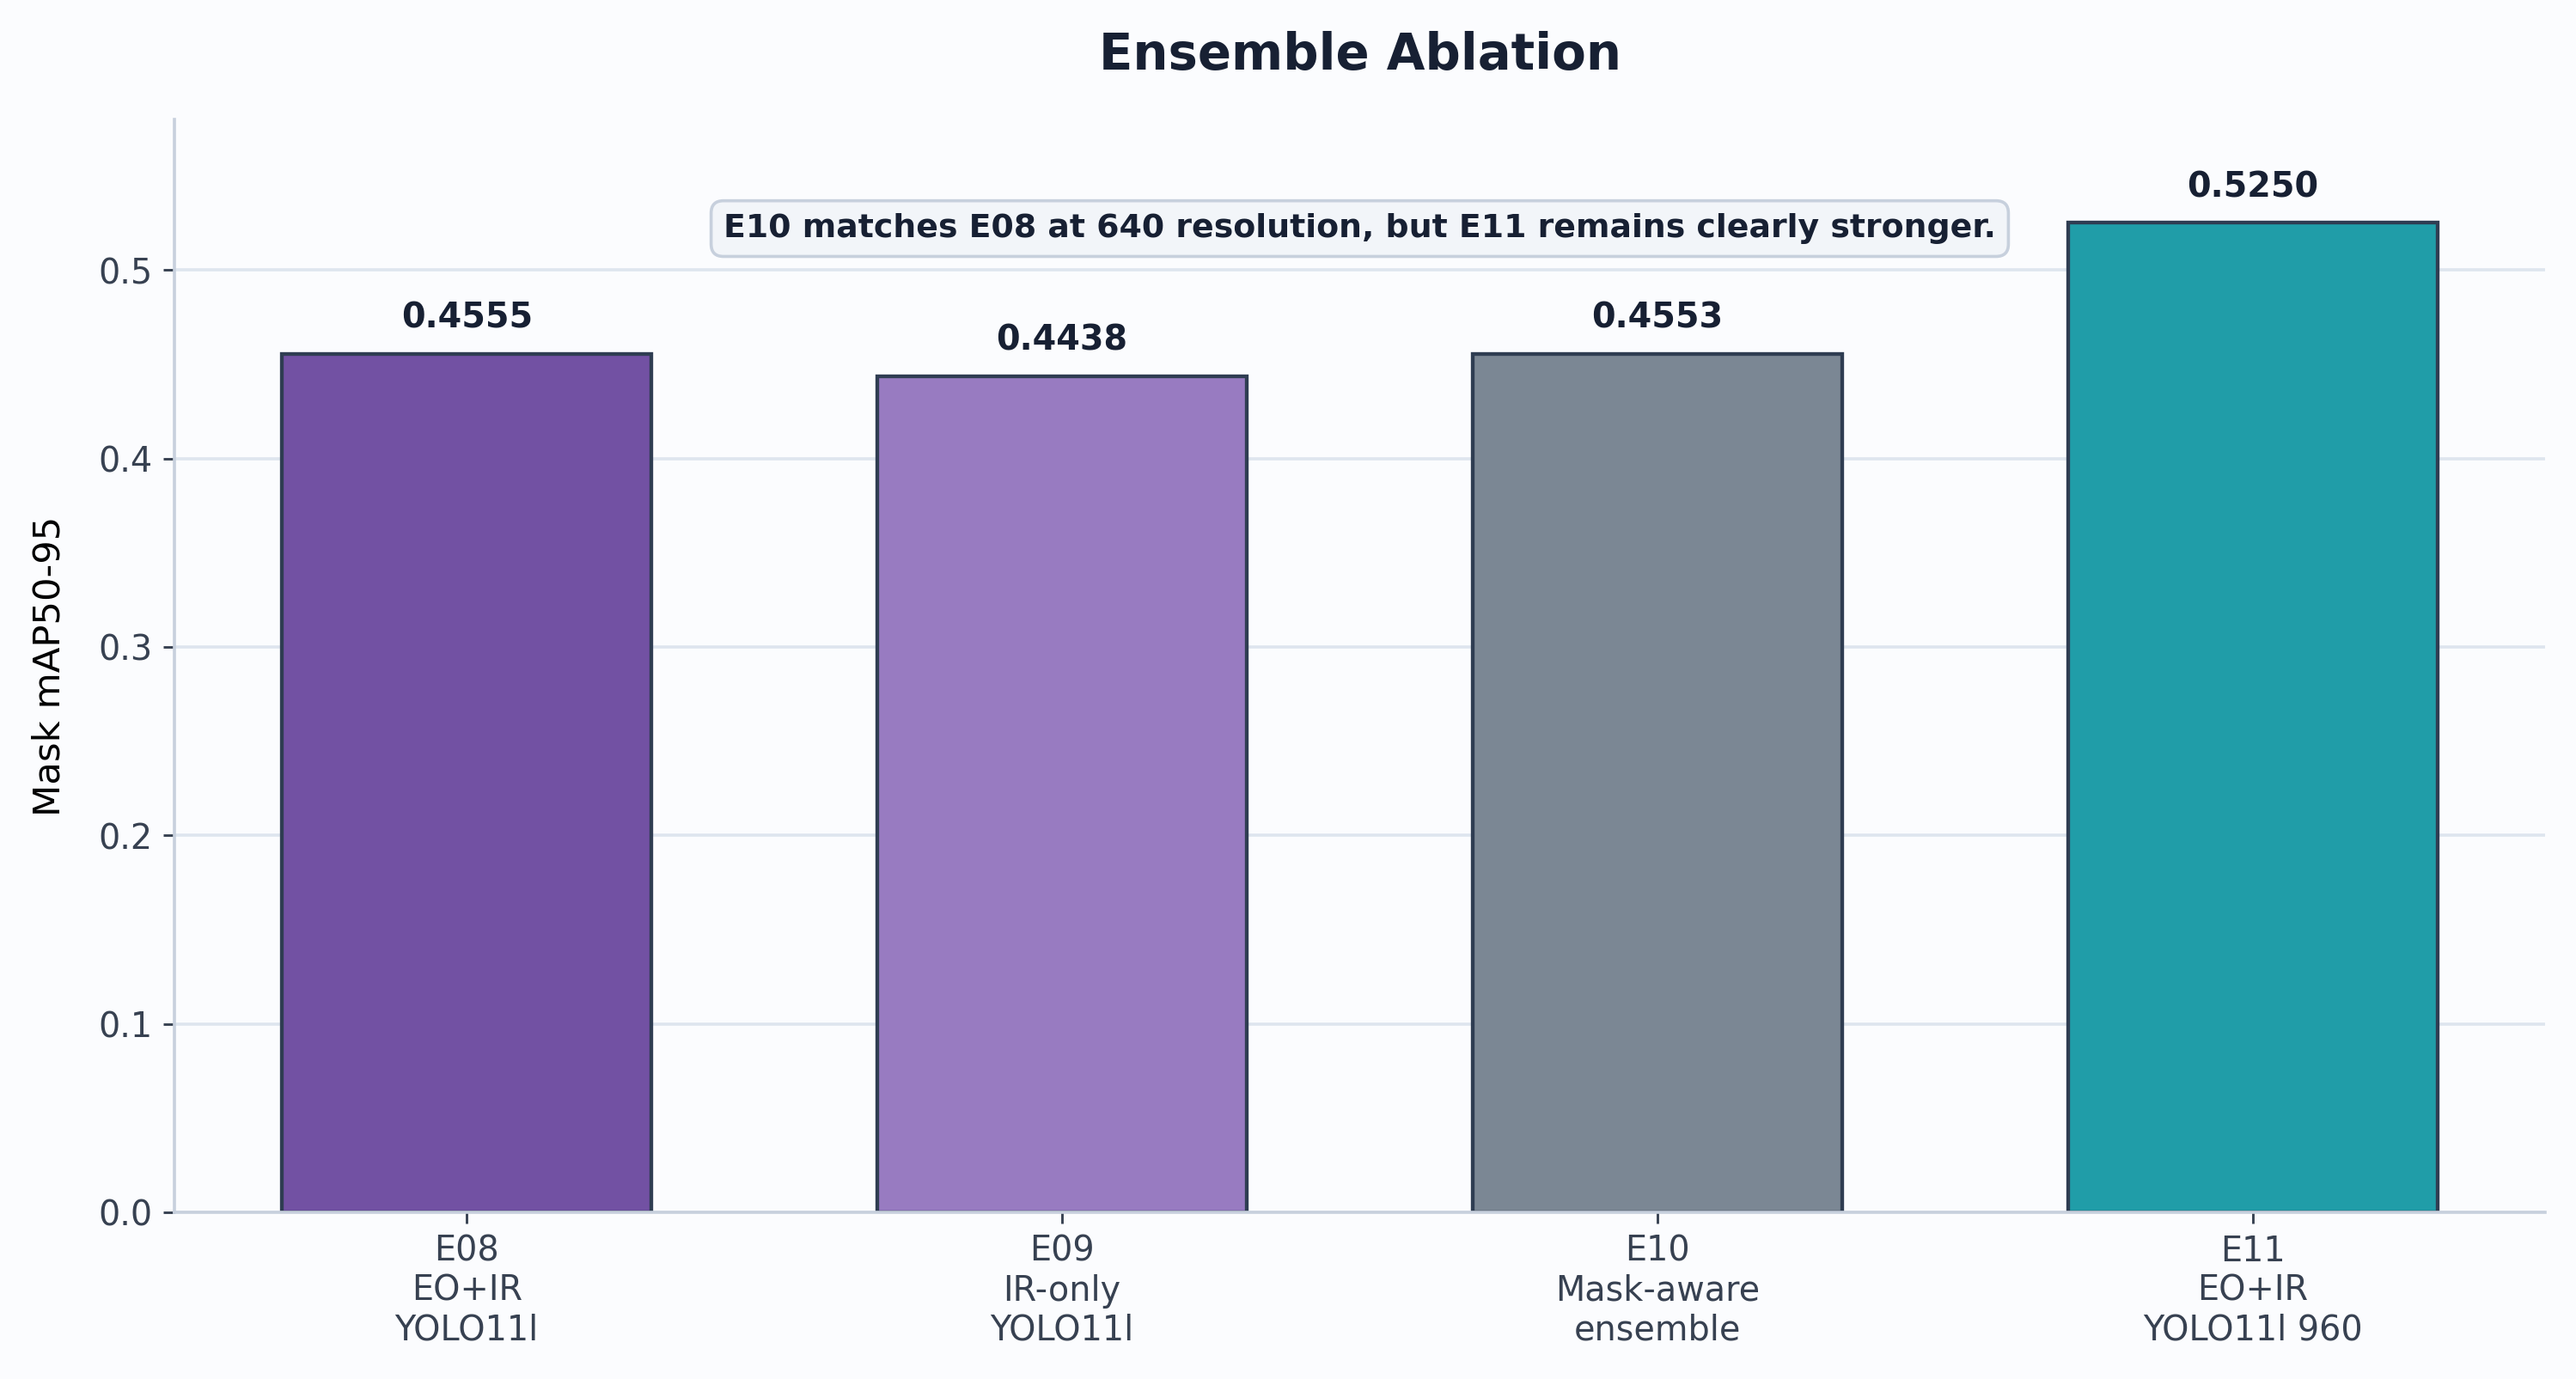
\includegraphics[width=\textwidth]{Figures/Chapter5/ensemble_ablation.png}%
}{%
\fbox{\parbox{0.92\textwidth}{\centering Placeholder for \texttt{ensemble\_ablation.png}}}%
}
\caption{Mask-aware ensemble ablation compared with strong single-model baselines.}
\label{fig:ensemble_ablation}
\end{figure}

This result shows that simple prediction-level ensembling does not necessarily improve segmentation mask quality. In this study, a strong high-resolution single model is more effective than the evaluated ensemble strategy.

\section{Complete IR-only Results}

Table \ref{tab:full_ir_results} summarizes all full experiments on IR-only validation. E11 is the best model under the primary metric, followed by E12. The lowest values belong to the EO-only and grayscale-domain baselines.

\begin{figure}[htbp]
\centering
\IfFileExists{Figures/Chapter5/ir_results_ranking.png}{%
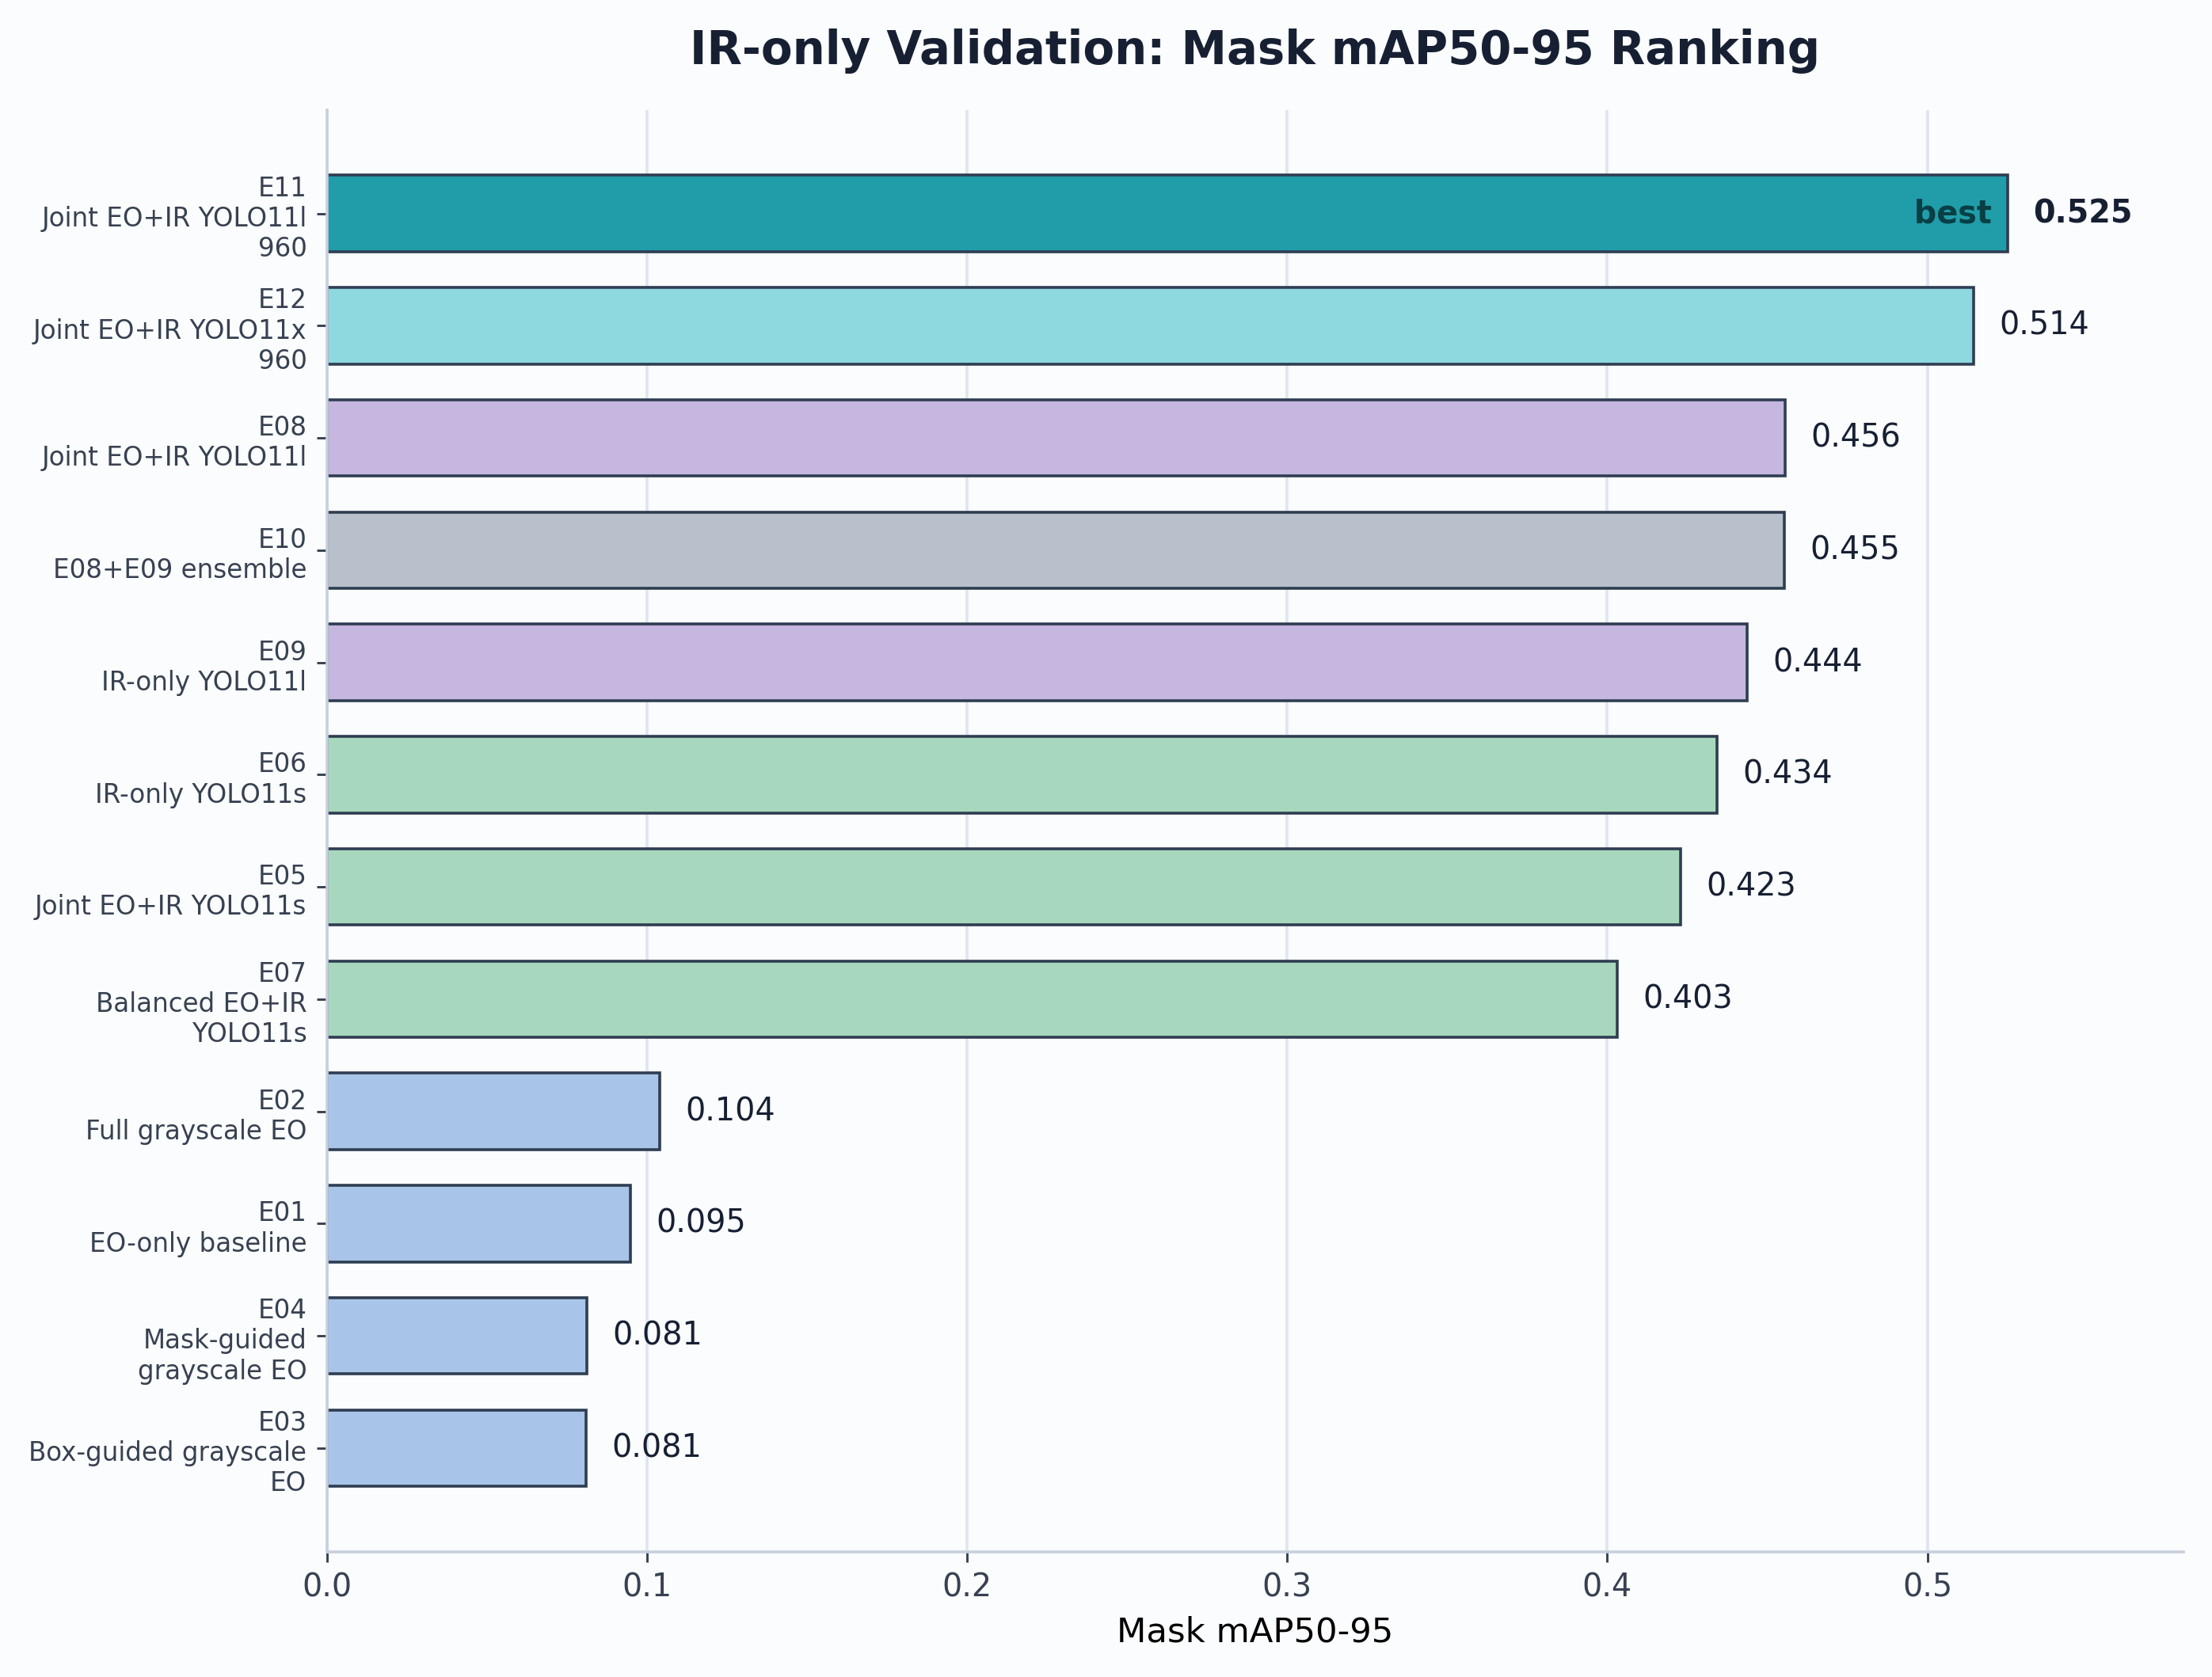
\includegraphics[width=\textwidth]{Figures/Chapter5/ir_results_ranking.png}%
}{%
\fbox{\parbox{0.92\textwidth}{\centering Placeholder for \texttt{ir\_results\_ranking.png}}}%
}
\caption{IR-only validation ranking of all full experiments using mask mAP50-95.}
\label{fig:ir_results_ranking}
\end{figure}

\begin{table}[h]
\centering
\caption{Complete IR-only validation results.}
\label{tab:full_ir_results}
\small
\begin{tabular}{llllrr}
\hline
\textbf{ID} & \textbf{Method} & \textbf{Model} & \textbf{Training Data} & \textbf{Mask mAP50} & \textbf{Mask mAP50-95} \\
\hline
E01 & EO-only baseline & YOLO11s-seg & EO & 0.2203 & 0.0948 \\
E02 & Full grayscale EO & YOLO11s-seg & EO gray & 0.2274 & 0.1040 \\
E03 & Box-guided grayscale EO & YOLO11s-seg & EO box-gray & 0.1972 & 0.0811 \\
E04 & Mask-guided grayscale EO & YOLO11s-seg & EO mask-gray & 0.2006 & 0.0812 \\
E05 & Joint EO+IR & YOLO11s-seg & EO+IR & 0.6691 & 0.4229 \\
E06 & IR-only supervised & YOLO11s-seg & IR & 0.6530 & 0.4342 \\
E07 & Balanced EO+IR & YOLO11s-seg & EO+IR balanced & 0.6407 & 0.4031 \\
E08 & Joint EO+IR large & YOLO11l-seg & EO+IR & 0.6968 & 0.4555 \\
E09 & IR-only large & YOLO11l-seg & IR & 0.6555 & 0.4438 \\
E10 & Mask-aware ensemble & 2x YOLO11l-seg & EO+IR + IR & 0.6910 & 0.4553 \\
E11 & Joint EO+IR high-res & YOLO11l-seg & EO+IR & 0.7025 & \textbf{0.5250} \\
E12 & Joint EO+IR high-res XL & YOLO11x-seg & EO+IR & \textbf{0.7041} & 0.5145 \\
\hline
\end{tabular}
\end{table}

\section{Complete Combined EO+IR Results}

Table \ref{tab:full_eo_ir_results} summarizes all full experiments on combined EO+IR validation. E12 achieves the best combined mask mAP50-95 score. E11 is the second strongest model and remains close to E12.

\begin{figure}[htbp]
\centering
\IfFileExists{Figures/Chapter5/combined_results_ranking.png}{%
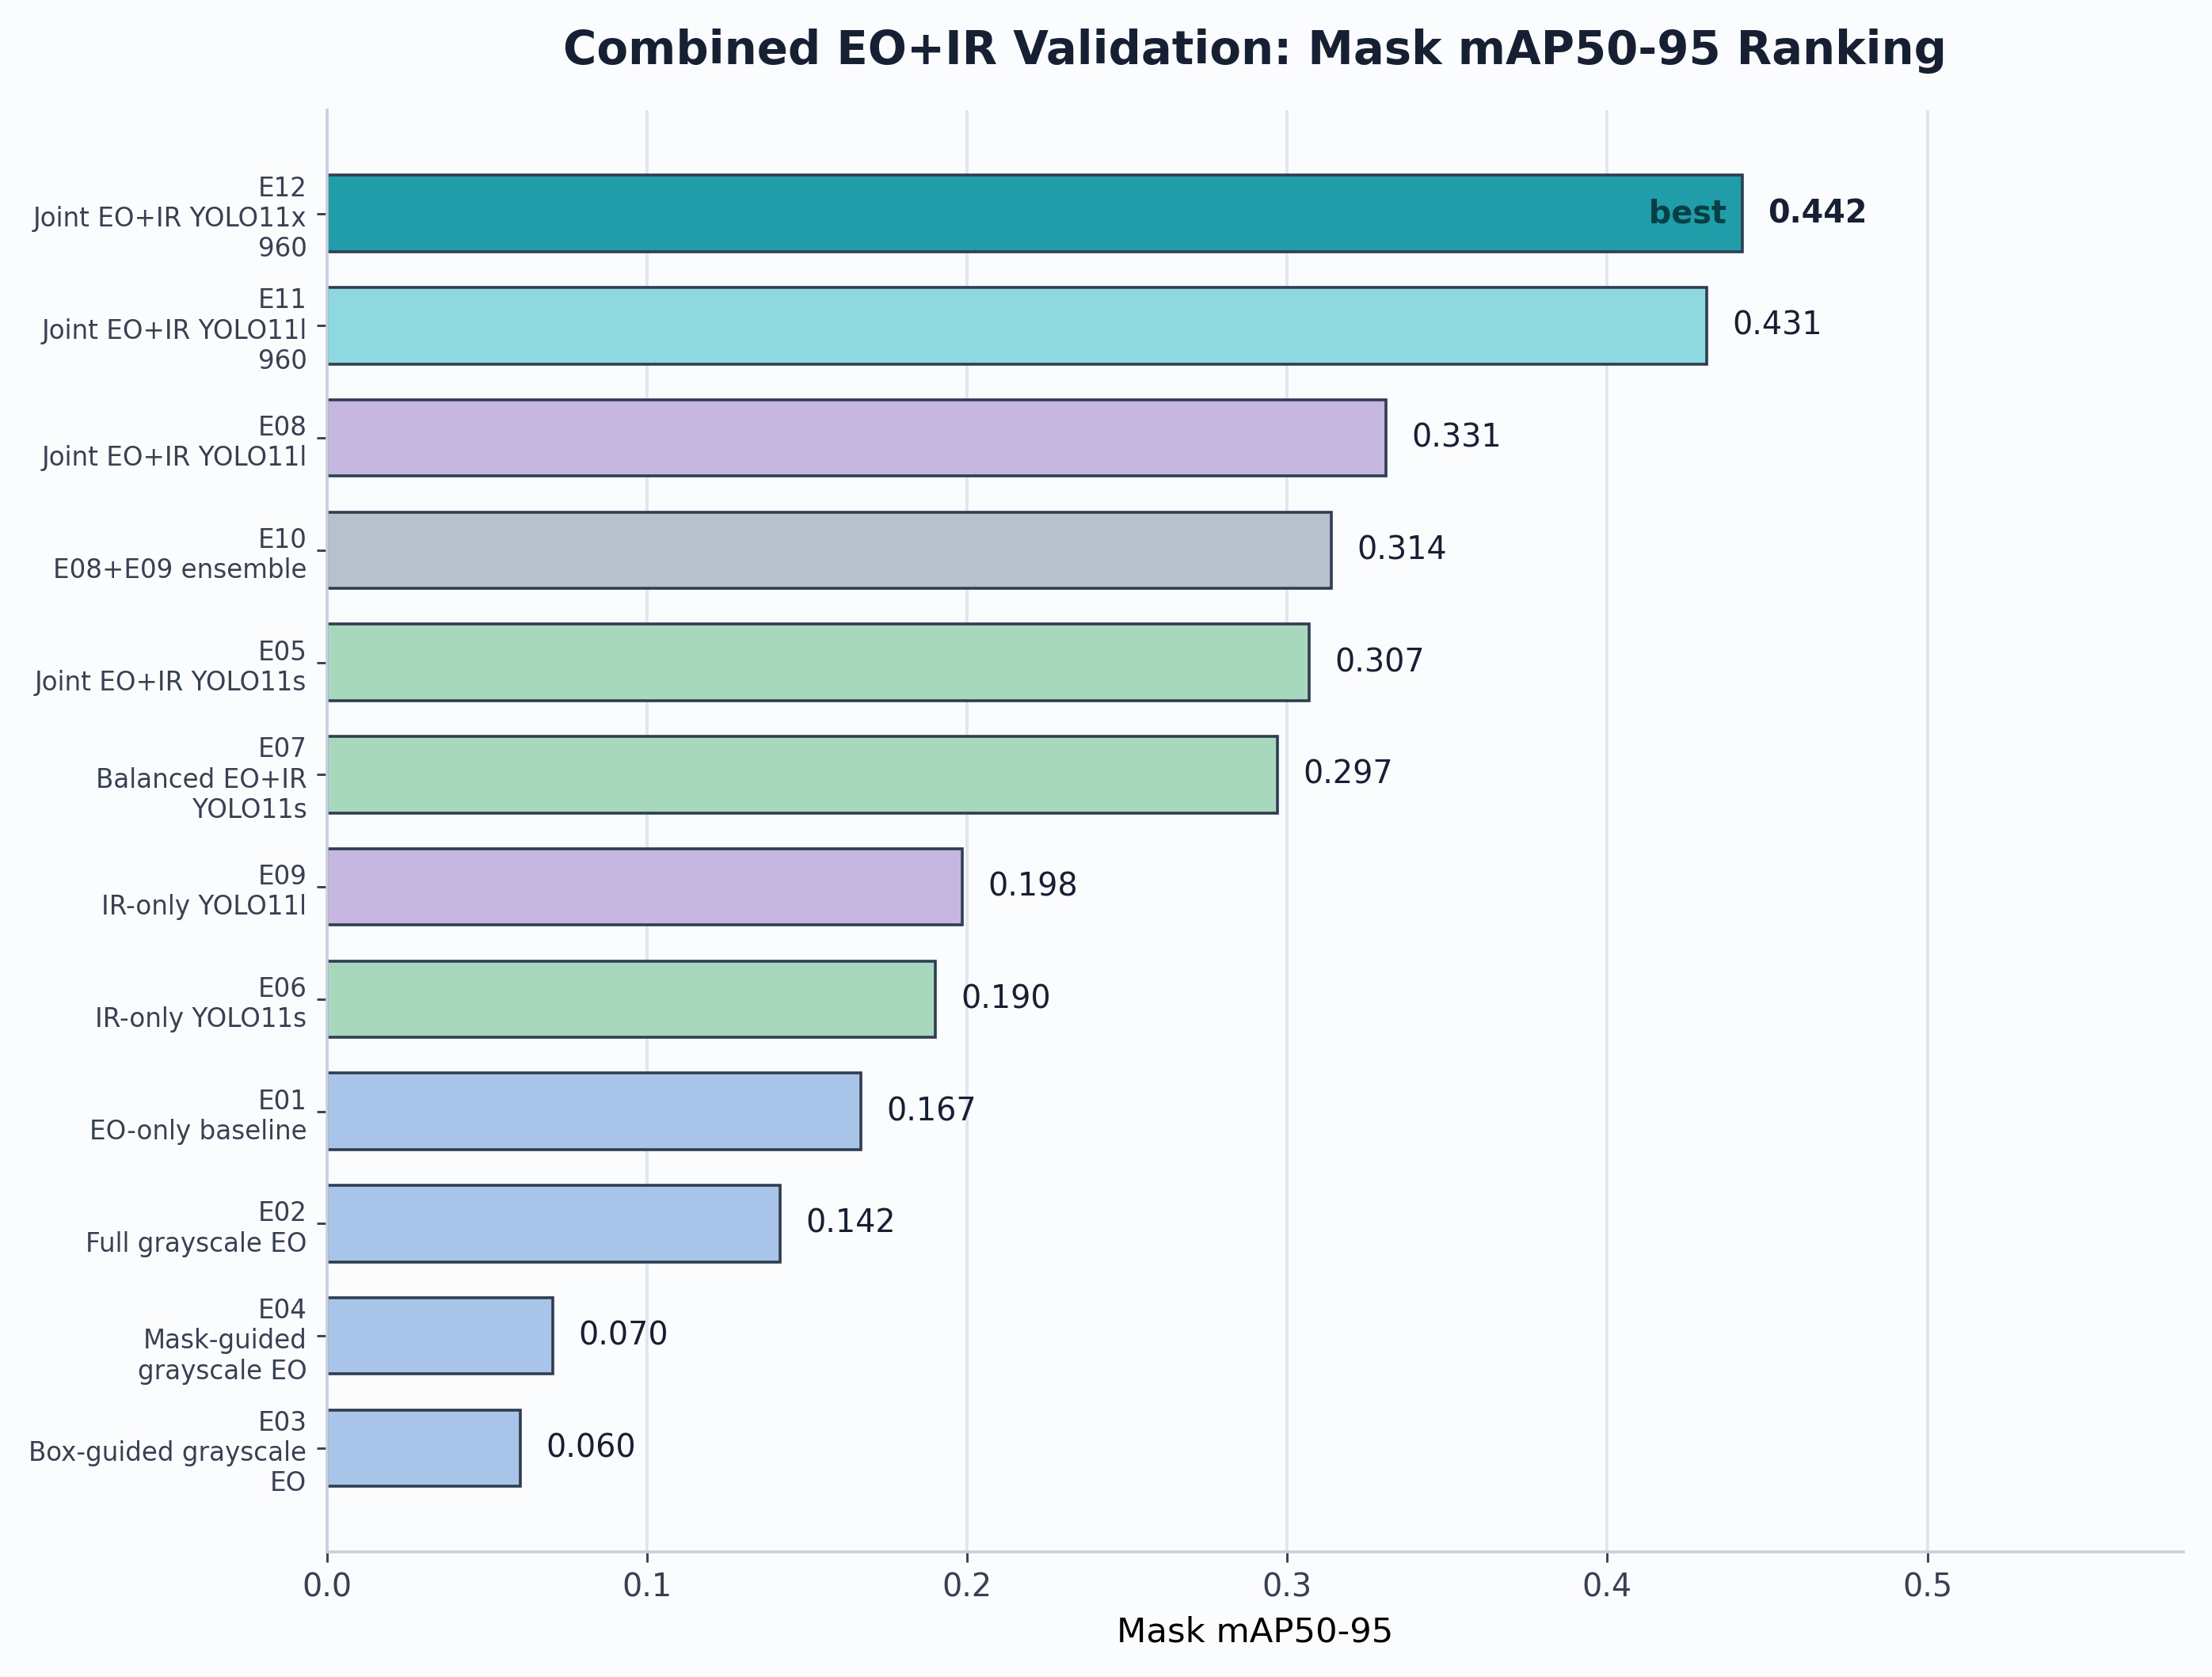
\includegraphics[width=\textwidth]{Figures/Chapter5/combined_results_ranking.png}%
}{%
\fbox{\parbox{0.92\textwidth}{\centering Placeholder for \texttt{combined\_results\_ranking.png}}}%
}
\caption{Combined EO+IR validation ranking using mask mAP50-95.}
\label{fig:combined_results_ranking}
\end{figure}

\begin{table}[h]
\centering
\caption{Complete combined EO+IR validation results.}
\label{tab:full_eo_ir_results}
\small
\begin{tabular}{llllrr}
\hline
\textbf{ID} & \textbf{Method} & \textbf{Model} & \textbf{Training Data} & \textbf{Mask mAP50} & \textbf{Mask mAP50-95} \\
\hline
E01 & EO-only baseline & YOLO11s-seg & EO & 0.3386 & 0.1669 \\
E02 & Full grayscale EO & YOLO11s-seg & EO gray & 0.2917 & 0.1417 \\
E03 & Box-guided grayscale EO & YOLO11s-seg & EO box-gray & 0.1427 & 0.0605 \\
E04 & Mask-guided grayscale EO & YOLO11s-seg & EO mask-gray & 0.1768 & 0.0705 \\
E05 & Joint EO+IR & YOLO11s-seg & EO+IR & 0.5483 & 0.3069 \\
E06 & IR-only supervised & YOLO11s-seg & IR & 0.3233 & 0.1902 \\
E07 & Balanced EO+IR & YOLO11s-seg & EO+IR balanced & 0.5251 & 0.2969 \\
E08 & Joint EO+IR large & YOLO11l-seg & EO+IR & 0.5823 & 0.3308 \\
E09 & IR-only large & YOLO11l-seg & IR & 0.3448 & 0.1984 \\
E10 & Mask-aware ensemble & 2x YOLO11l-seg & EO+IR + IR & 0.5462 & 0.3139 \\
E11 & Joint EO+IR high-res & YOLO11l-seg & EO+IR & 0.6163 & 0.4310 \\
E12 & Joint EO+IR high-res XL & YOLO11x-seg & EO+IR & \textbf{0.6463} & \textbf{0.4422} \\
\hline
\end{tabular}
\end{table}

\section{Final Model Selection}

The results support two final model recommendations. If the target is primary IR-domain segmentation, E11 is preferred because it obtains the highest IR mask mAP50-95 score of 0.5250. If the target is combined EO+IR robustness, E12 is preferred because it obtains the highest combined EO+IR mask mAP50-95 score of 0.4422.

\begin{figure}[htbp]
\centering
\IfFileExists{Figures/Chapter5/final_model_recommendation.png}{%
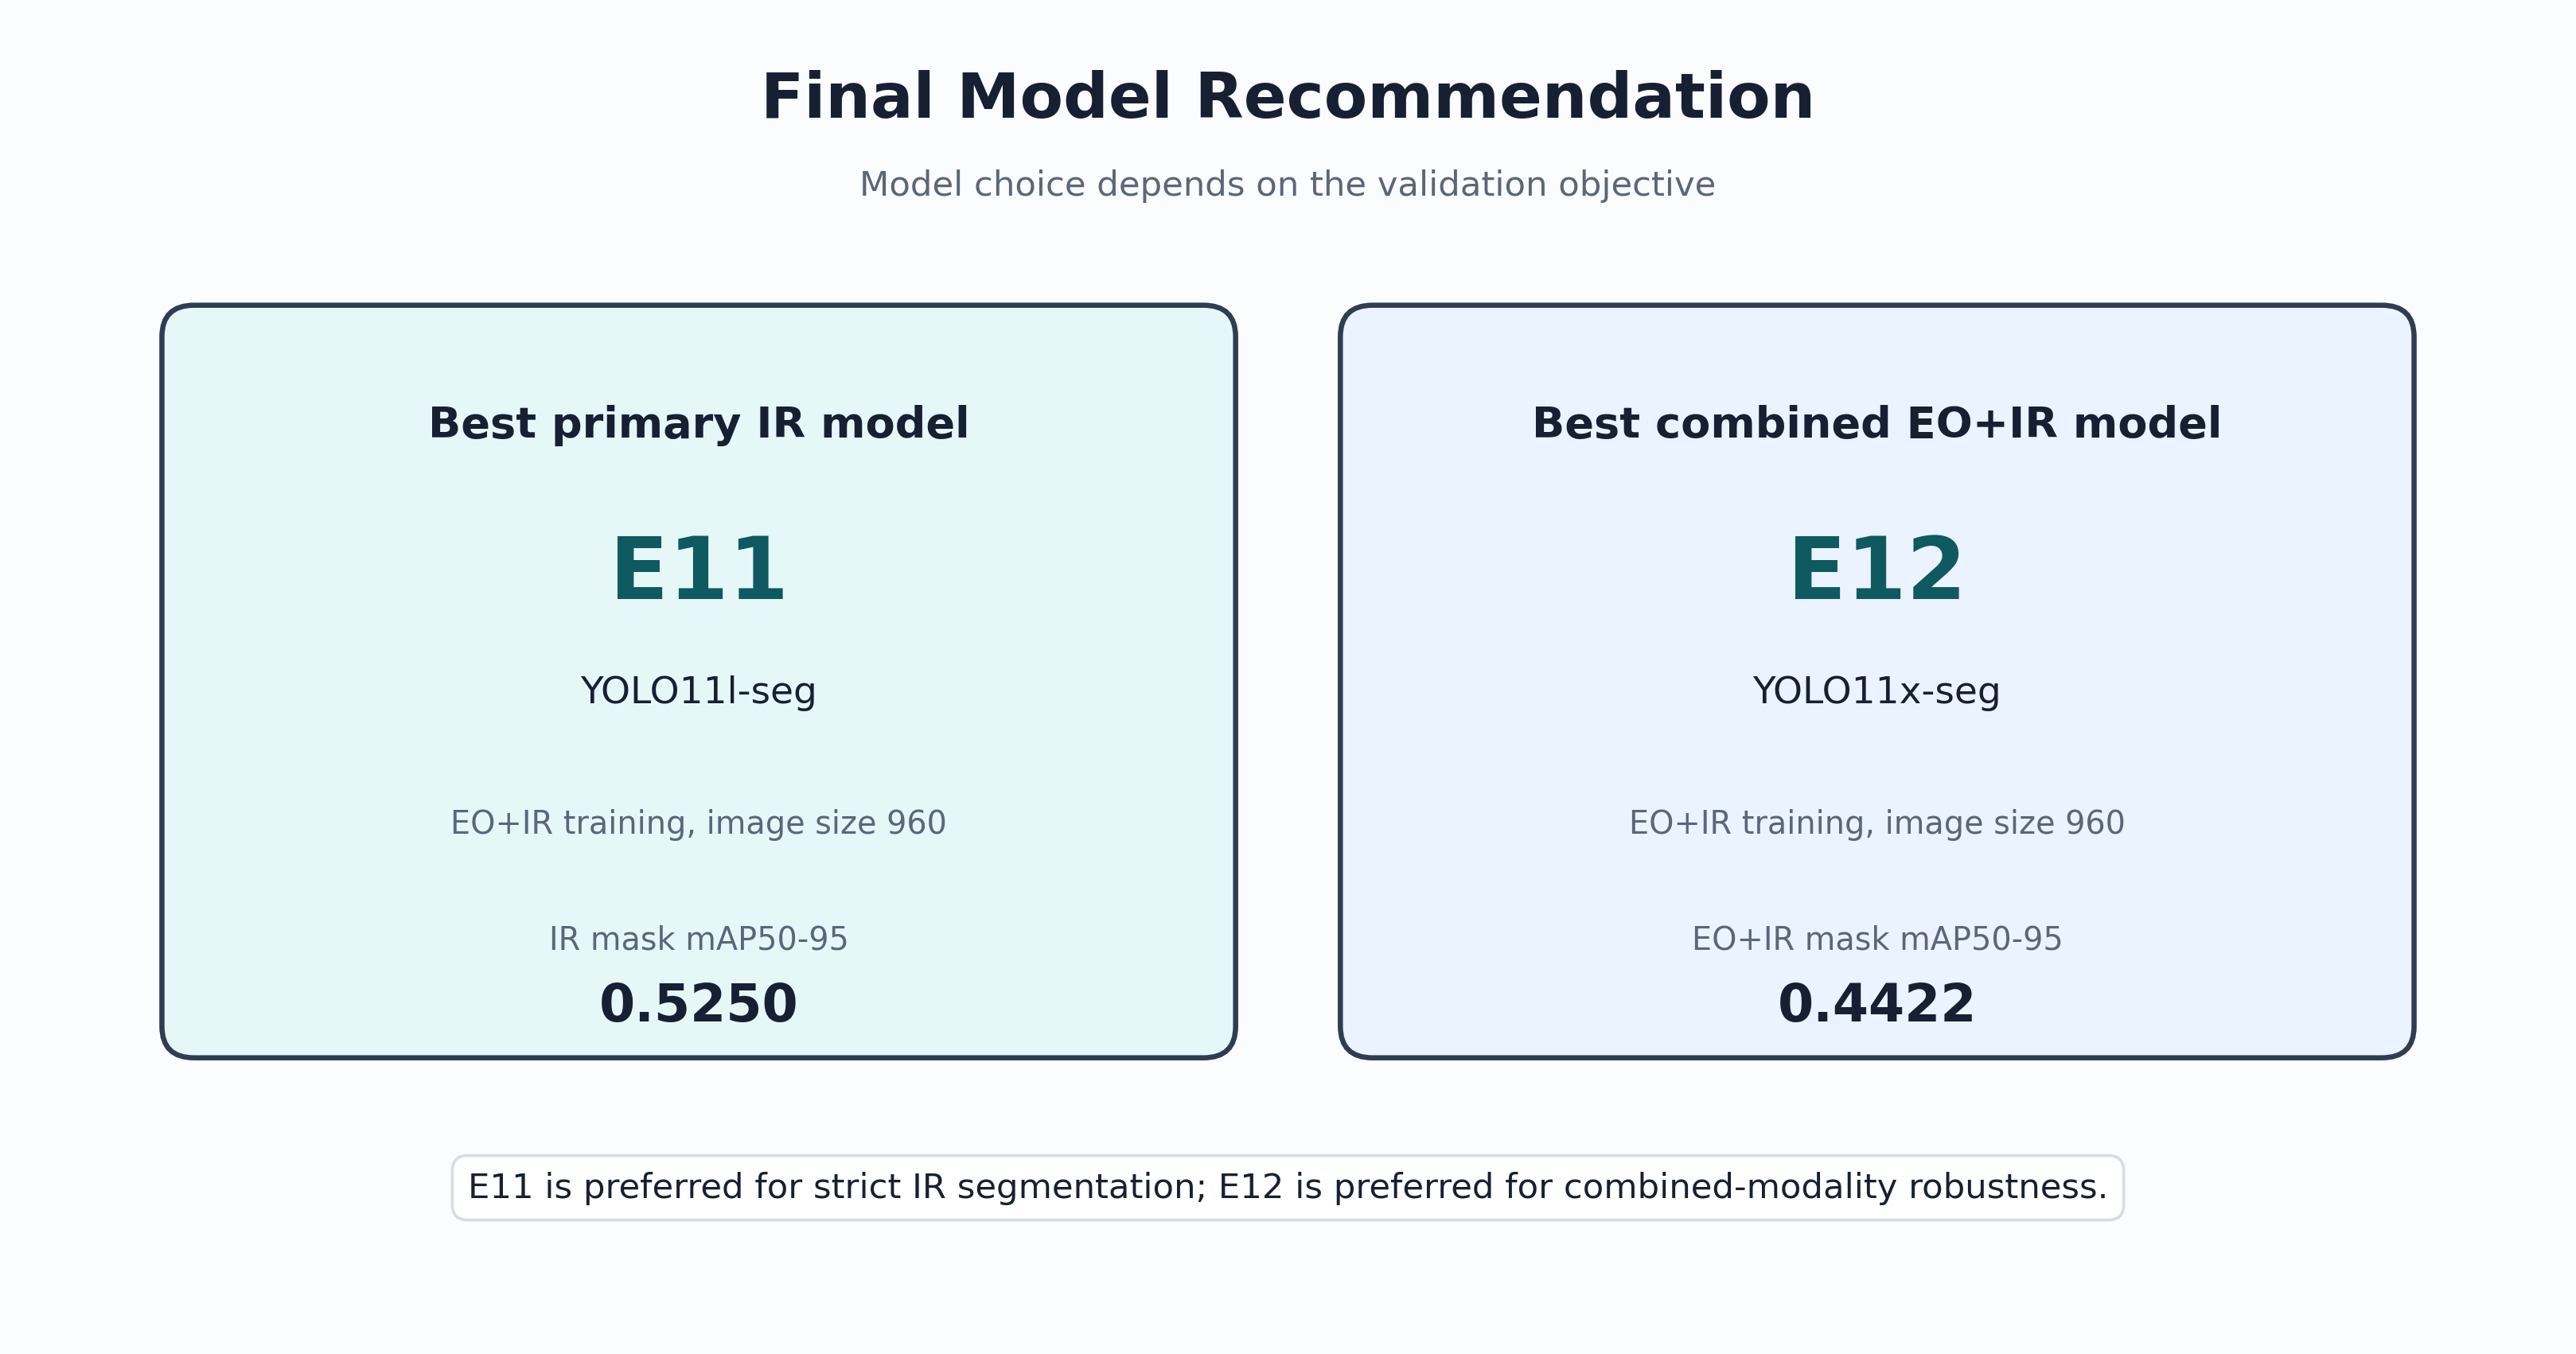
\includegraphics[width=\textwidth]{Figures/Chapter5/final_model_recommendation.png}%
}{%
\fbox{\parbox{0.92\textwidth}{\centering Placeholder for \texttt{final\_model\_recommendation.png}}}%
}
\caption{Summary of the best model choices for IR-only and combined EO+IR evaluation.}
\label{fig:final_model_recommendation}
\end{figure}

This distinction is important because the best model depends on the deployment objective. E11 gives the strongest strict mask performance on IR images, while E12 provides the best combined-modality performance. Therefore, the dissertation does not present one model as universally best. Instead, it reports the most suitable model under each evaluation requirement.

\section{Discussion}

The experimental results lead to several observations. First, EO-only segmentation models do not transfer well to IR validation. This confirms that the EO-to-IR gap is significant for segmentation. Second, grayscale-domain transformations provide only limited improvement. This suggests that removing color information is not enough to reproduce IR appearance.

Third, real IR supervision changes the result substantially. The jump from E01 to E05 is the largest improvement in the experiment sequence. This indicates that target-domain labels are highly valuable for IR segmentation. Fourth, larger YOLO models improve performance, but the benefit is smaller than the gain from adding IR supervision. Fifth, high-resolution training provides the cleanest improvement in strict mask quality, especially for the YOLO11l model. This is consistent with the small-object nature of aerial traffic imagery.

Finally, the ensemble experiment shows that combining models at prediction level is not automatically better than training a stronger single model. For this dataset and model family, high-resolution joint training is more effective than the evaluated mask-aware ensemble.

\section{Chapter Summary}

This chapter presented the experimental results and analysis. EO-only and grayscale-domain baselines were weak on IR segmentation. Adding real IR supervision produced the largest performance improvement. Increasing model size improved performance further, and increasing input resolution to 960 produced the strongest strict IR mask result. The mask-aware ensemble did not outperform the best high-resolution single model. Overall, E11 is the strongest primary IR segmentation model, while E12 is the strongest combined EO+IR model. The next chapter concludes the dissertation and discusses limitations and future work.
